\newpage

\section{Las fuerzas del mercado de la oferta y de la demanda}

\subsection{¿Qué es un mercado?}
Un {\bf mercado} es un grupo de compradores y vendedores de un bien o sevicio en particular. Los
compradores son el grupo que determina la demanda del producto y los vendedires on el grupo que determina la oferta de dicho producto.
\subsection{¿Qué es la competencia?}
En la mayoría de los mercados en la economía, cada uno de los compradores sabe que hay varios vendedores a los que se les puede comprar y cada uno de los vendedores está consciente de que su producto es similar al ofrecido por otros vendedores. 
\par El termino \underline{mercado conpetitivo} se refiere a un mercado en el que hay múltiples compradores y vendedores y, por tanto, individualmente ninguno de ellos tiene un impacto significativo en el precio de mercado. En este capítulo trabajaremos con un mercado perfectamente competitivo. 
Para llegar a esta forma de competencia, el mercado debe tener dos caractetísticas:
\begin{enumerate}
\item{Los bienes que se venden deben de ser exactamente los mismos(Bienes Homogéneos)}
\item{Los compradores y vendedores son tan numerosos que ninguno puede, por sí solo, influir en el precio del bien en el mercado}
\item{Existe perfecta información entre los compradores y vendedores}
\item{No existen costos de transporte}
\end{enumerate}
Debido a que en los mercados perfectamente competitivos los compradores y vendedores deben aceptar el precio que el mercado determina, se dice que ambos son {\bf tomadores de precios}. Cuando no hay competencia perfecta podemos estar en un caso de:

\begingroup
\setlength{\tabcolsep}{5pt} % Default value: 6pt
\renewcommand{\arraystretch}{1.5} % Default value: 1
\begin{center}
\begin{tabular}{p{1.7cm}|p{11cm}}
{\bf Monopolio}& Un vendedor, y el vendedor controla el precio\\
{\bf Oligopolio}& Pocos vendedores y competencia no siempre es agresiva (manipulación precio)
\end{tabular}
\end{center}
\endgroup

\subsection{La Demanda}
\subsubsection{Los cuatro conceptos más importantes}
\begin{description}
\item[Cantidad de Demanda] En un bien determinado, es la cantidad que de ese bien están dispuestos a adquirir los compradores
\item[Bien Normal] Se entiende por bien normal, aquel que al aumentar la renta del individuo, también aumenta su demanda.
\item[Bien Inferior] Se entiende por bien inferior, aquel que al aumentar la renta del individuo, este cambia sus preferencias demandando otros productos.
\item[Bien Sustituto] Se entiende por bien sustituo, aquel que al aumentar el precio del bien, el consumidor cambia sus preferencias demandando otros productos.
\item[Bien Complementario] Se entiende por bien complementario, aquel que al disminuir la demanda de un item, tambien lo hace el segundo bien.
\item[Ley de la demanda] Esta establece que la cantidad demandada de un bien cae cuando el precio del bien sube, y todo lo demás constante. La cantidad demandada siempre está relacionada negativamente con el precio. 
\item[Tabla de la demanda] Muestra la relacíon que existe entre el precio de un bien y la cantidad demandada, cuando todo lo demás permanece constante
\item[Curva de la demanda] Esta gráfica la relación entre el precio del bien y la cantidad de demanda. Se entiende que la cantidad demandada tendra directa relación con la renta del individuo. Otros factores que determinan la demanda, son los Gustos y preferencias de las personas. Junto a las expectativas y disposición a gastar en el tiempo
\end{description}

\subsubsection{La demanda del mercado frente a la demanda individual}
La {\bf demanda del mercado} se refiere a la suma de todas las demandas individuales de un bien o servicio en particular. Gráficamente, las curvas de demanda individuales se suman horizontalmente para obtener la curva de demanda del mercado.

\subsubsection{Desplazamiento en la cuerva de la demanda}
\begin{wrapfigure}{r}{0.4\textwidth} %this figure will be at the right
    \centering
    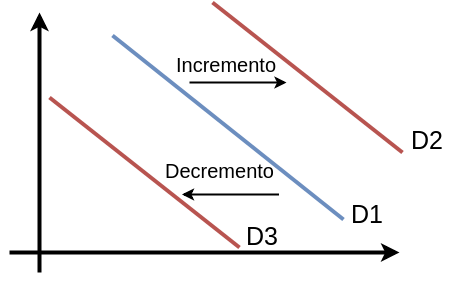
\includegraphics[width=0.3\textwidth]{images/demand1.png}
\end{wrapfigure}

Si ocurre algo que altere algo altere la cantidad demandada a un precio dado, automáticamente la cuerva de la demanda se desplazará. A un precio dadocualquier cambio que incremente la cantidad demadnada desplazará la cuerva de la demanda a la derecha y esto reflejará un \textit{incremento en la demanda}. Por el contrario, cualquier cambio que reduzca la cantidad demanda a todo precio desplazará a la curva de la demanda a la izquierda. A esto se le conoce como \textit{decremento en la demanda} Un cambio en el precio es considerado un movimiento de {largo plazo}.\\

Las variables de mayor importancia que pueden producir un desplzamiento en la curva de demanda:
\begin{itemize}
\item{{\bf Ingresos}: Si la demanda de un bien disminuye, cuando se reduce el ingreso, se dice que es un {\bf bien normal}. No todos los bienes son normales. Si la demanda de un bien aumenta cuando el ingreso disminuye, se dice que es un {\bf bien inferior}}
\item{{\bf Precios de bienes relacionados}: Cuando la reducción en el precio de un bien reduce la demadna de otro, se dice que los {\bf bienes son sustitutos}. Ahora, cuando la reducción en el precio de un bien incrementa la demanda de otro, se dice que los {\bf bienes son complementarios}}
\item{Gustos}
\item{{\bf Expectativas}: Las expectivas que sobre el futuro tengan las personas pueden afectar, en el presente, la demanda de bienes y servicios}
\item{Número de compradores}
\end{itemize}

\subsection{La Oferta - (Supply)}

\subsubsection{Los cuatro conceptos más importantes}
\begin{description}
\item[Cantidad de Ofrecida] En un bien o servicio es la cantidad que los vendedores quieren y pueden vender.
\item[Ley de la Oferta] Es la relación entre el precio y la cantidad ofrecida. Con todo constante, cuando el precio aumenta, la cantidad ifrecidad de dicho bien también aumenta y cuando el precio disminuye, la cantidad que se ofrece de dicho bien también disminuye.
\item[Tabla de la oferta] Muestra la realación que existe entre el precio de un bien y la cantidad ofrecida, manteniendo constante todo lo que pueda influir en la cantidad que los productores quieren vender
\item[Curva de la demanda] Esta gráfica la relación entre el precio del bien y la cantidad de demanda  
\end{description}

\subsubsection{La oferta del mercado de la oferta}
Así como la demanda del mercado es la suma de la demanda de todos los compradores, la orferta del mercado es la suma de todo lo ofrecido por los vendedores.
\par Al igual que en el caso de las curvas de la demanda, las curvas de la oferta se suman horizontalmente para obtener la cuerva de la oferta del mercado.

\subsubsection{Deplazamientos en la curva de la oferta}
Existen muchas variables que desplazan la curva de la oferta. He aquí algunas de las más importantes

\begin{itemize}
\item{{\bf Precios de los insumos}: La oferta de un bien se relaciona negativamente con el precio de los insumos utilizados para producir dicho bien.}
\item{Tecnología}
\item{Expectativas}
\item{Número de vendedores}
\end{itemize}

\newpage

\subsection{Oferta y demanda juntas}
Ahora combinamos ambas curvas para ver cómo se determinan el precio y la cantidad de un bien vendido en un mercado.
Hay un punto en el cual ambas curvas se intersecan. Este punto se llama \underline{equilibrio de mercado}.
Por lo tanto, el \textbf{equilibrio} se da cuando el precio marcado ha llegado al nivel en el cual la cantidad ofrecida equivale a la cantidad demandada.

\par Las acciones de compradores y vendedores mueven naturalemente los mercados hacia el equilibrio de la oferta y la demanda. Para entender por qué, considere lo siguiente:


\begin{figure}[hbt!]
    \centering
    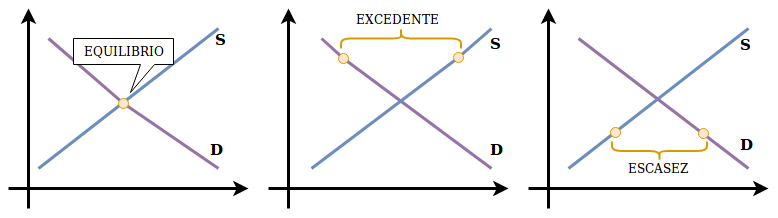
\includegraphics[scale=0.6]{images/char4.png}
\end{figure}